\section{Reprise des clients dans Comp@ssV4}

\subsection{Deux groupes de clients: ``Cluster" et ``Référentiel Groupe"}

Dans le contexte du projet Comp@ssV4, tous les clients ne seront pas repris au niveau du référentiel commun groupe.\\
Les autres seront définis uniquement au niveau de l'instance "Cluster", c'est à dire le système SAP sur lequel fonctionne le site Valeo car ces clients lui sont propres et ne sont pas partagés avec les autres sites.
\begin{figure}[H]
    \centering
    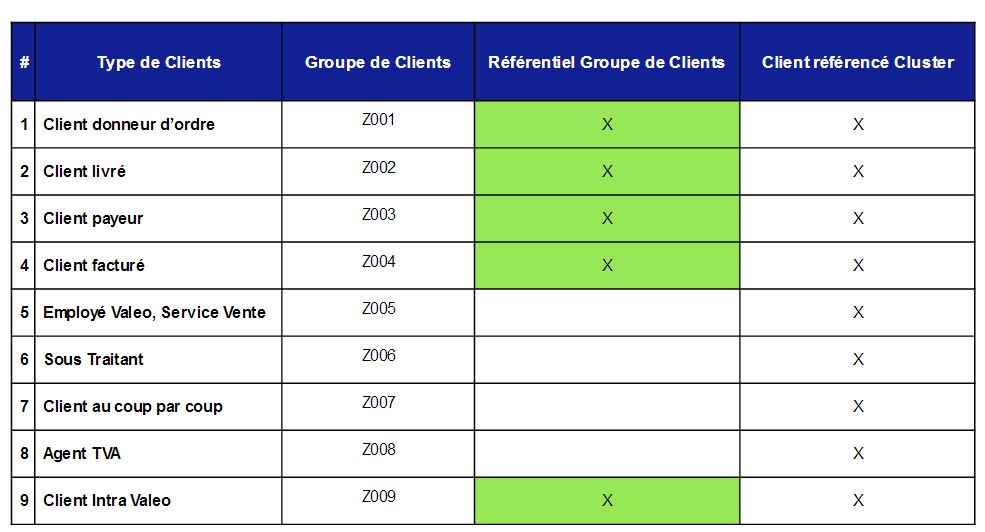
\includegraphics[height=6.5cm]{compassCustomerGroup.jpg}
	\caption{Reprise des clients Comp@ssV2 - Referentiel Groupe vs Cluster}\label{image.compassCustomerGroup} 
\end{figure}

\subsection{Cadre de reprise d'un client}
Il n'est pas cohérent de reprendre tous les clients des systèmes SAP de tout Valeo. En effet, certains ne sont plus actifs, n'existent plus, ont déménagés, ou n'ont tout simplement plus aucune activité avec Valeo.

Ainsi chaque site Valeo, devra choisir parmi ses clients comp@ssV2, ceux qui répondent à l'ensemble des critères suivant:

\begin{itemize}\itemsep4pt
	\item Tous les clients non marqués ``à supprimer" (On ne supprime jamais rien, on applique des marqueurs de suppression dans un système ERP: soucis de traçabilité).
	\item Tous les clients ayant effectué une commande durant les 2 dernières années.
	\item Tous les clients avec une commande non clôturée (en cours ou en litige ou en attente de paiement)
\end{itemize}

Tous ces filtres sont ajoutés à l'outil d'extraction que nous utilisons: \href{http://www.informatica.com/us/SAP/}{\textbf{Informatica}}.


\clearpage

\section{Une nouvelle codification client}

\subsection{Presentation de la nouvelle codification}

\begin{figure}[H]
    \centering
    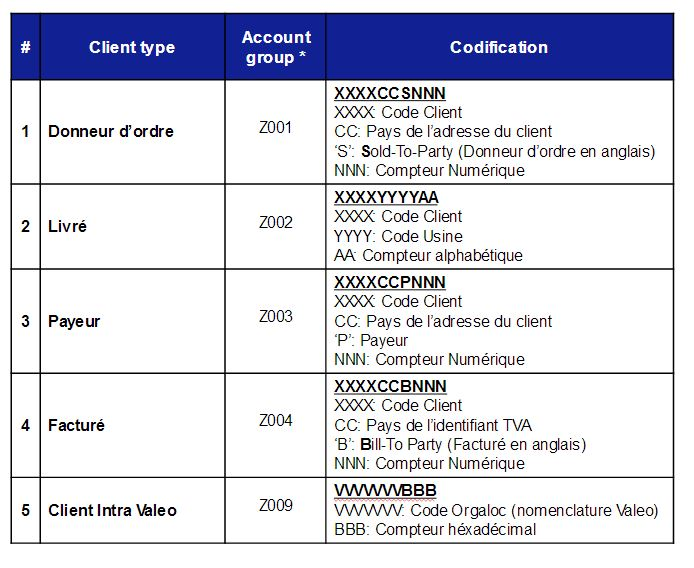
\includegraphics[height=11cm]{compassCustomerCodification.jpg}
	\caption{Nouvelle Codification Client du système Comp@ssV4 - Codification Unifiée}\label{image.compassCustomerCodification} 
\end{figure}

La codification Comp@ssV4 assure que chaque client ne correspondra qu'à\textbf{ une seule fonction partenaire} et non plusieurs comme cela était parfois le cas dans Comp@ssV2. Ainsi un client du groupe Z001 n'aura qu'une fonction partenaire : AG au lieu de AG/WE/RE et RG, comme parfois, dans Comp@ssV2.

La codification Comp@ssV4 définit le \textbf{code Client étant unique}. Ainsi deux clients différents auront un code client différent (exemple: \textit{Renault et BMW}), par contre deux clients du même Groupe (au sens entreprise) auront un code client commun (exemple: Renault Douai et Renault Compiegne).

La codification Comp@ssV4 définie le code usine de manière unique quelque soit l'entreprise et l'usine. Ainsi deux usines ne peuvent avoir en aucun cas le même numéro (Exemple: Renault Douai, Renault Compiegne et BMW Munich auront tous les trois un code Usine obligatoirement différent).

\section{Processus de migration de Comp@ssV2 à Comp@ssV4}

\begin{figure}[H]
    \centering
    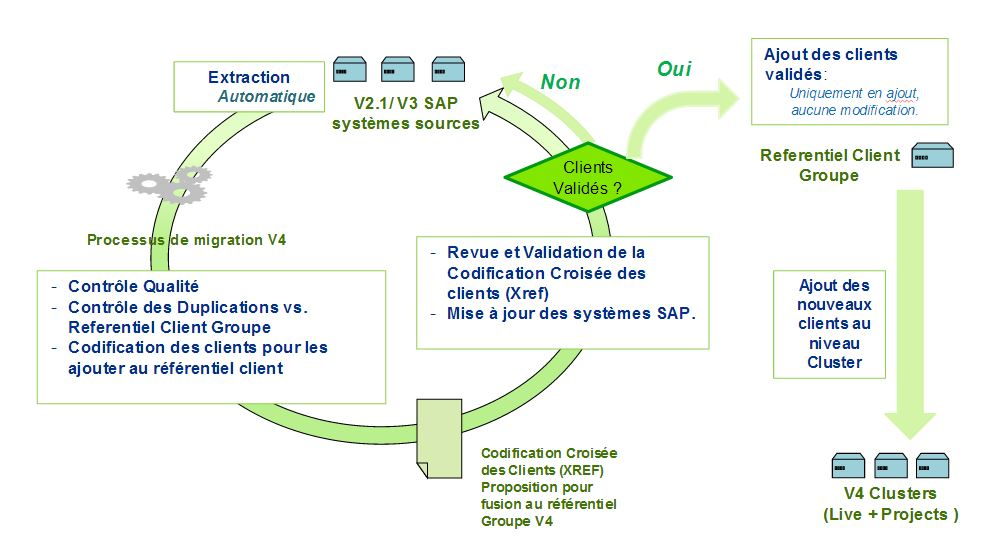
\includegraphics[height=12.5cm, angle =90]{compassV4MigrationProcess.jpg}
	\caption{Processus de migration de Comp@ssV2 à Comp@ssV4}\label{image.compassV4MigrationProcess} 
\end{figure}


